\section{Introducción}
	En el presente laboratorio se espera dar las bases de la teoría de las comunicaciones para la demodulación de una radio FM y aplicarlas sobre un dispositivo físico.
Para ello se toma como referencia el libro \emph{Principles of Communications} \cite{PrinciplesofCommunications}.

La modulación de FM se trata de una modulación angular no lineal y idealmente se basa en transmitir el mensaje en la fase de la portadora (logrando una desviación de face según el mensaje) y la amplitud de la portadora mantenerla constante. Esto es, la señal modulada que sera transmitida por el canal se traduce en:
$$
	x_c (t) = A_c \cos \left( 2 \pi f_c t + 2 \pi k_f \int_{-\infty}^{t} m(\lambda) d\lambda \right)
$$

Donde $k_f$ es la constante desviación de frecuencia y es definido como:
$$
	k_f = \frac{\Delta f}{max|m(t)|}
$$


\section{Desarrollo}
En la demodulación se trata de reconstruir el mensaje $m(t)$ a partir de la señal que recibe la antena, que como se mencionó anteriormente es $x_c(t)$.
Para ello se utilizó el lenguaje python con las siguientes librerías para la implementación digital del circuito:
\begin{itemize}
	\item \texttt{rtlsdr}: Contiene funciones para poder controlar y usar el dongle SDR, véase \cite{pyrtlsdr}.
	\item \texttt{numpy}: Biblioteca de funciones matemáticas de alto nivel para operar con vectores o matrices
	\item \texttt{scipy}: También es una librería pero se basa más en operaciones que se utilizan en el procesamiento de señales y puntualmente con la sub librería \texttt{io} es posible realizar operaciones como guardar o abrir un archivo. 
	\item \texttt{matplotlib}: Es utilizado para generar gráficos que serón exportados a formato pdf.
	\item \texttt{sounddevice}: Es módulo de reproducción de audio, que sirve también para sreaming.
\end{itemize}

Se facilita una guía de instalación y uso de los scripts en el apéndice \ref{ap:guia} donde se pueden encontrar los pasos para recrear lo estudiado en el presente informe.

\subsection{Generador de una muestra de FM}\label{sec:sample-generator}
El archivo \texttt{sample.py} contiene el algoritmo para generar una muestra de la estación de radio \sampleFM MHz, el cual utiliza las funciones de \texttt{utils.py} para demodular la señal que se obtiene del dongle.

El primer paso es tomar las muestras, para ello se llama a la función \emph{GetSample}, la cual se inicializa los parámetros necesarios para el rtlsdr y toma N muestras con una cierta ganancia \emph{gain}.

La estación en cuestión se encuentra centrada en \emph{f\_offset} de tal manera de evitar interferencias en continua es decir en frecuencia cero. Esto ocurre porque al muestrear la señal provoca que la misma no tenga exactamente media cero. 
La figura \ref{fig:xc_offset_spectrum} muestra el espectro de la señal obtenida del dispositivo.
\begin{figure}[ht!]
	\centering
	\includegraphics[scale=0.7]{../xc_offset_spectrum.pdf}
	\caption{Espectro de la muestra capturada.}
	\label{fig:xc_offset_spectrum}
\end{figure}

Posteriormente se pasa a banda base usando la función \emph{ToBaseBand}, esta función lo que hace es multiplicar la señal por una exponencial, lo que se traduce en el espectro como un desplazamiento en frecuencia, quedando la señal $x_c$ centrada en frecuencia cero. Es decir:
$$
	x_b = x_c \cdot e^{-j 2 \pi f_{o_s}} \quad \quad f_{o_s} = \frac{f_{offset}}{f_s}
$$
Se puede observar el cambio en la figura \ref{fig:x_baseband_spectrum}, y su correspondiente DEP en la figura \ref{fig:x_baseband_DEP}.
\begin{figure}[ht!]
	\centering
	\includegraphics[scale=0.7]{../x_baseband_spectrum.pdf}
	\caption{Señal $x_c$ en banda base, es decir $x_b$.}
	\label{fig:x_baseband_spectrum}
\end{figure}

\begin{figure}[ht!]
	\centering
	\includegraphics[scale=0.8]{../xb_DEP.pdf}
	\caption{Densidad espectral de potencia la señal $x_b$.}
	\label{fig:x_baseband_DEP}
\end{figure}

Ahora que se tiene la señal $x_b$, señal en banda base, se procede a realizar el filtrado y diezmado para que entre otras cosas no se sume ruido ni parte de otros canales al siguiente paso que es demodular.
La función \emph{FilterAndDownSample} en el archivo \texttt{utils.py} tiene este propósito, en ella se calculan los coeficiente adecuados para armar un filtro con las características mostradas en la figura \ref{fig:filter_charac}, sabiendo que el ancho de banda de los canales de radios comerciales es de $f_{bw} = \canalBW \mbox{kHz}$.

Se puede observar en el apéndice \ref{ap:utils.py} (línea \ref{code:remezFunction}) la función \emph{remez}\footnote{De la librería \texttt{scipy.signal}, véase \href{https://docs.scipy.org/doc/scipy/reference/generated/scipy.signal.remez.html}{línk}} que es utilizada para la creación del filtro, el cual calcula los coeficientes del mismo de una respuesta de impulso finito (FIR) cuya función de transferencia minimiza el error máximo entre la ganancia deseada y la ganancia realizada en las bandas de frecuencia especificadas utilizando el algoritmo de intercambio Remez.
En resumen, se detallan a continuación los cuatro parámetros que recibe dicha función para confeccionarlos: 
\begin{itemize}
	\item $1^{er}$ parámetro: \emph{numtaps}, traps es el número de términos en el filtro, o el orden de filtro más uno.
	\item $2^{do}$ parámetro: es una secuencia que contiene los bordes de la banda.
	En el ejemplo se tomaron intervalo de cero a el ancho de banda deseado y una caída del filtro que posee un $\caidaFiltro$ del ancho de pasa bajos. 
	\item $3^{er}$ parámetro: Una ponderación relativa para dar a cada región de banda. La longitud del peso tiene que ser la mitad de la longitud segundo parámetro.
	Es decir en el ejemplo se le multiplica por la unidad a las frecuencias que van de cero a $f_{bw}$ y un valor muy chico a las frecuencias que van de $f_{bw} + \caidaFiltro$ a $f_s/2$.
	\item $4^{to}$ parámetro: Frecuencia de muestreo.
\end{itemize}

La figura \ref{fig:x_downsample_spectrum} muestra el resultado de filtrar utilizando los coeficiente de Remez de orden 50 y de diezmar la señal $x_b$.

Antes de demodular, se puede observar en la figura \ref{fig:x_downsample_constelation} el espacio de señal de fm. 

\begin{figure}[ht!]
	\centering
	\includegraphics[scale=0.8]{../filter_charac.pdf}
	\caption{Respuesta en frecuencia, que caracteriza el filtro pre-demodulación.}
	\label{fig:filter_charac}
\end{figure}

\begin{figure}[ht!]
	\centering
	\includegraphics[scale=0.8]{../x_downsample_spectrum.pdf}
	\caption{Señal filtrada y diezmada.}
	\label{fig:x_downsample_spectrum}
\end{figure}

\begin{figure}[ht!]
	\centering
	\includegraphics[scale=0.8]{../x_downsample_constelation.pdf}
	\caption{Gráfico de constelación de señal filtrada y diezmada.}
	\label{fig:x_downsample_constelation}
\end{figure}

\subsubsection{Demodulación}
La señal resultante de los pasos anteriores todavía no esta demodulada sino que se acondiciona la señal ya que es posible que anteriormente contenga parte de otros canales, entre otros aspectos. 

Para demodular la señal se optó por un tipo de discriminador de frecuencia llamado discriminador polar.
Este mide la diferencia de fase entre muestras consecutivas de una señal FM muestreada de forma compleja. Esto se traduce en realizar la siguiente operación (línea \ref{code:demod-conj} del apéndice \ref{ap:utils.py}):
$$
	x_d[n] = x[n] \cdot \overline{x}[n-1]
$$
Donde $\overline{x}$ es el conjugado de $x$ y luego tomar el angulo de $x_d[n]$ (línea \ref{code:demod-angle} del apéndice \ref{ap:utils.py}):
$$
	y_d[n] = \arctan\Big( \frac{I}{R} \Big)
$$

Más específicamente, toma muestras sucesivas de valores complejos y multiplica la nueva muestra por el conjugado de la muestra anterior. Luego toma el ángulo de este valor complejo. Esta resulta ser la frecuencia instantánea de la señal de FM muestreada.

\subsubsection{Densidad espectral de potencia}

\begin{figure}[ht!]
	\centering
	\includegraphics[scale=0.8]{../yd_DEP.pdf}
	\caption{Densidad espectral de potencia la señal (yd) resultante diferenciando las distintas partes.}
	\label{fig:yd-DEP}
\end{figure}

El resultado de todos los procesos anteriormente mencionados, se puede observar en la figura \ref{fig:yd-DEP}.
Se puede notar cuatro zonas de interés con diferentes colores\footnote{Para más información ingrese al siguiente \href{https://en.wikipedia.org/wiki/FM\_broadcasting\#Other\_subcarrier\_services}{link}}:
% CALCULOS
\FPeval{\leftLimitStereo}{clip(\centeredStereo - \bandStereo)}
\FPeval{\rightLimitStereo}{clip(\centeredStereo + \bandStereo)}

\begin{itemize}
	\item Color rojo: Señal mono, es el de mayor interés, va de 0 a \limitMono kHz.
	\item Color verde: En la transmisión FM estéreo, el tono piloto centrada en \pilotTone kHz, indica que hay una información estereofónica. El receptor duplica la frecuencia del tono piloto (\centeredStereo kHz) y lo usa como frecuencia de referencia para demodular la información estéreo.
	\item Color naranja: Señal stereo, la banda de \leftLimitStereo k a \centeredStereo k Hz se encuentra el canal izquierdo y de \centeredStereo k a \rightLimitStereo kHz el canal derecho.
	\item Color cyan: Una subportadora centrada en \digitalCarrier kHz, se usa para transmitir una señal de sistema de datos de radio digital de ancho de banda angosta, que proporciona características adicionales de la estación de radio.
\end{itemize}

\subsubsection{Deénfasis}
El deénfasis (o de-emphasis en ingles\footnote{Para mas información véase \href{https://en.wikipedia.org/wiki/FM\_broadcasting\#Pre-emphasis\_and_de-emphasis}{link}.}) consiste en disminuir las altas frecuencias en el receptor ya que el transmisor envía la señal con una ganancia elevada en comparación a las bajas frecuencias, esto se debe a que el ruido afecta más a las altas frecuencias en FM\footnote{Si decea saber más sobre cuanto afecta el ruido en la señal FM puede encontrar en la sección 8.8.3 del libro \cite{PrinciplesofCommunications}.}
.
Para ellos físicamente se utiliza un circuito RC y en america latina se utiliza una contante $\tau = 75$ para dicho propósito.

El código que realiza esta tarea se encuentra en el apéndice \ref{ap:utils.py}, línea \ref{code:FilterPreEmphasis}.


\subsection{Radio Streaming}\label{sec:radio}

El objetivo de esta sección es tratar de reproducir la señal recibida por alguna emisora en tiempo real, es decir como una radio comercial. Cabe destacar que se utilizó la librerías gráfica Qt versión 4 para el desarrollo de la GUI.

Para ello se tienen algunas consideraciones respecto de la sección anterior, los cuales se mencionarán a continuación.
Las librerías usadas en python como el lenguaje en sí no tienen paralelismo implícito, esto es, si se quiere realizar dos tareas a la vez (en simultaneo) se debe usar la librería \emph{threading}, que contiene algoritmo de bajo nivel para el aprovechamiento del hardware.
Se destacan dos tareas que deben ser ejecutadas por separado de forma simultanea y sin interrupción, capturar las muestras con el dongle y reproducir el audio, por lo tanto se optó por crear tres threads o hilos (el tercero es para la demodulación y procesamiento de la señal), teniendo en cuenta esto último el tiempo de procesamiento $T_p$ tine que ser considerablemente menor a los tiempos de captura $T_c$ y de reproducción $T_r$, es decir:
$$
	T_p \ll T_c = \frac{N}{f_s}
$$
Donde $f_s$ es la frecuencia de muestreo; si esto no se cumple se obtendrá interrupciones al escuchar ya que el buffer de reproducción de audio estará vacía.

En el archivo llamado \texttt{radio.py} (véase apéndice \ref{ap:radio.py}) se implementa la radio en cuestión. Se pueden observar los tres hilos de ejecución: 
\begin{itemize}
	\item Capturadora: en línea \ref{code:thread-capture}, a diferencia de como se captura las muestras en la sección anterior, en primer lugar se sustituyo la función \emph{read\_samples} por lo que que hace realmente\footnote{Puede verlo en el siguiente \href{https://github.com/roger-/pyrtlsdr/blob/master/rtlsdr/rtlsdr.py\#L480}{línk}.}.
	Por otro, se toman de a muestras mas pequeñas por limitaciones del hardware (USB y dongle) y se concatena las muestras para procesar el conjunto. 
	
	\item Procesamiento: en línea \ref{code:thread-processing}, realiza lo mismo que en la sección anterior salvo por deénfasis que no se realiza, ya este caso se trata de optimizar el uso de variables y uso del procesador.

	\item Reproducción: en línea \ref{code:thread-reproduce}, este hilo tiene la particularidad de usar la clase \emph{OutputStream} de la librería sounddevice en la que es posible almacenar muestras de audio en un buffer y reproducirlas rápidamente.
\end{itemize}

Por ultimo, los archivos de la GUI que usa las funciones de la radio son: \texttt{qt.py} en el que se ejecuta la ventana de control. El archivo \texttt{windows.py} configuran las variables de la interfaz (tamaño de ventana, titulo de ventana, barra de estado, etc) y cumple la función de nexo entre la radio en sí y los botones que se encuentran en el panel central. Y el archivo \texttt{centerWidget.py} crea los botones junto con el deslizable de frecuencia los agrupa de forma tal como se muestra en la figura \ref{fig:gui}.

\begin{figure}[ht!]
	\centering
	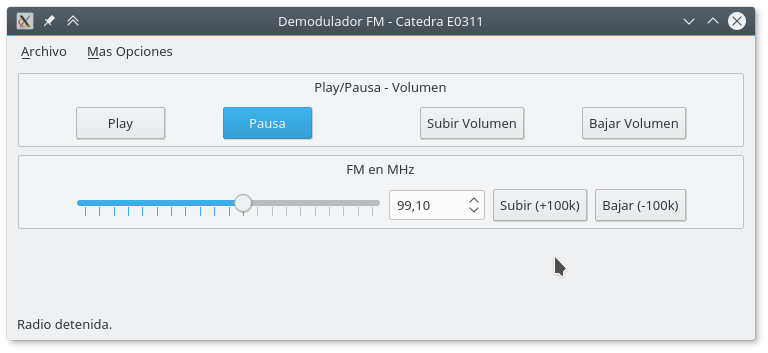
\includegraphics[scale=0.7]{./imagenes/gui.png}
	\caption{Diseño de la GUI con Qt4}
	\label{fig:gui}
\end{figure}

\section{Conclusiones}

Se puede llegar a la conclusión de que con el procesamiento digital genera resultados muchos mas rápidos y de menor costo si se hubiera hecho de forma analógica.
Sin embargo, el lenguaje python, que es un lenguaje interpretado, no tiene suficiente rendimiento para optimizar los cálculos, lo que conlleva a un mal desempeño para el procesamiento de señales en tiempo real. En contrapartida existe lenguajes capaces de lograr el objetivo como Matlab, que a pesar de que es interpretado posee esta optimizado) o de mas bajo nivel como C entre otros.

Existen módulos pendientes o en fase beta para la radio streaming que son: volumen (fase beta), cascada de la potencia promedio o waterfall FM, entre otros.
